\documentclass[a4paper,10pt]{memoir}
\usepackage[italian]{babel}
\usepackage{wrapfig}
\usepackage[pdftex]{graphicx}
\usepackage{graphviz}
\usepackage{graphicx}
\usepackage{listingsutf8}
\usepackage{amsmath}
\usepackage{afterpage}
\usepackage{subfig}
\usepackage{quoting, lipsum}
\usepackage{float}

%Define the listing package
\usepackage{listings} %code highlighter
\usepackage{color} %use color
\definecolor{mygreen}{rgb}{0,0.6,0}
\definecolor{mygray}{rgb}{0.5,0.5,0.5}
\definecolor{mymauve}{rgb}{0.58,0,0.82}
 
%Customize a bit the look
\lstset{ %
backgroundcolor=\color{white}, % choose the background color; you must add \usepackage{color} or \usepackage{xcolor}
basicstyle=\footnotesize, % the size of the fonts that are used for the code
breakatwhitespace=false, % sets if automatic breaks should only happen at whitespace
breaklines=true, % sets automatic line breaking
captionpos=b, % sets the caption-position to bottom
commentstyle=\color{mygreen}, % comment style
deletekeywords={...}, % if you want to delete keywords from the given language
escapeinside={\%*}{*)}, % if you want to add LaTeX within your code
extendedchars=true, % lets you use non-ASCII characters; for 8-bits encodings only, does not work with UTF-8
frame=single, % adds a frame around the code
keepspaces=true, % keeps spaces in text, useful for keeping indentation of code (possibly needs columns=flexible)
keywordstyle=\color{blue}, % keyword style
% language=Octave, % the language of the code
morekeywords={*,...}, % if you want to add more keywords to the set
numbers=left, % where to put the line-numbers; possible values are (none, left, right)
numbersep=5pt, % how far the line-numbers are from the code
numberstyle=\tiny\color{mygray}, % the style that is used for the line-numbers
rulecolor=\color{black}, % if not set, the frame-color may be changed on line-breaks within not-black text (e.g. comments (green here))
showspaces=false, % show spaces everywhere adding particular underscores; it overrides 'showstringspaces'
showstringspaces=false, % underline spaces within strings only
showtabs=false, % show tabs within strings adding particular underscores
stepnumber=1, % the step between two line-numbers. If it's 1, each line will be numbered
stringstyle=\color{mymauve}, % string literal style
tabsize=2, % sets default tabsize to 2 spaces
title=\lstname % show the filename of files included with \lstinputlisting; also try caption instead of title
}
%END of listing package%
 
\definecolor{darkgray}{rgb}{.4,.4,.4}
\definecolor{purple}{rgb}{0.65, 0.12, 0.82}
 
%define Javascript language
\lstdefinelanguage{JavaScript}{
keywords={typeof, new, true, false, catch, function, return, null, catch, switch, var, if, in, while, do, else, case, break},
keywordstyle=\color{blue}\bfseries,
ndkeywords={class, export, boolean, throw, implements, import, this},
ndkeywordstyle=\color{darkgray}\bfseries,
identifierstyle=\color{black},
sensitive=false,
comment=[l]{//},
morecomment=[s]{/*}{*/},
commentstyle=\color{purple}\ttfamily,
stringstyle=\color{red}\ttfamily,
morestring=[b]',
morestring=[b]"
}

\lstdefinelanguage{docker}{
  keywords={FROM, RUN, COPY, ADD, ENTRYPOINT, CMD,  ENV, ARG, WORKDIR, EXPOSE, LABEL, USER, VOLUME, STOPSIGNAL, ONBUILD, MAINTAINER},
  keywordstyle=\color{blue}\bfseries,
  identifierstyle=\color{black},
  sensitive=false,
  comment=[l]{\#},
  commentstyle=\color{purple}\ttfamily,
  stringstyle=\color{red}\ttfamily,
  morestring=[b]',
  morestring=[b]"
}

\lstdefinelanguage{docker-compose-2}{
  keywords={version, volumes, services},
  keywordstyle=\color{blue}\bfseries,
  keywords=[2]{image, environment, ports, container_name, ports, links, build},
  keywordstyle=[2]\color{blue}\bfseries,
  identifierstyle=\color{black},
  sensitive=false,
  comment=[l]{\#},
  commentstyle=\color{purple}\ttfamily,
  stringstyle=\color{red}\ttfamily,
  morestring=[b]',
  morestring=[b]"
}

\lstset{
language=JavaScript,
extendedchars=true,
basicstyle=\footnotesize\ttfamily,
showstringspaces=false,
showspaces=false,
numbers=left,
numberstyle=\footnotesize,
numbersep=9pt,
tabsize=2,
breaklines=true,
showtabs=false,
captionpos=b
}

\newcommand\blankpage{%
    \null
    \thispagestyle{empty}%
    \addtocounter{page}{-1}%
    \newpage}

\usepackage[chapter]{minted}
\usepackage{adjustbox}
\usepackage{hyperref}
\hypersetup{
  colorlinks   = true,    % Colours links instead of ugly boxes
  urlcolor     = black,    % Colour for external hyperlinks
  linkcolor    = black,    % Colour of internal links
  citecolor    = black      % Colour of citations
}

% import package
\usepackage{FrontespizioSapienza}

\pagestyle{plain}%%to insert the number of the page

% declare info
\FSSTitolo{Titolo}
\FSSFacolta{Ingegneria dell'Informazione, Informatica e Statistica}
\FSSCorso{Informatica}

\FSSCandidato{Edoardo Ottavianelli}
\FSSMatricola{1756005}
\FSSRelatore{Emanuele Panizzi}
\FSSCorrelatore{}
\FSSAnnoAccademico{2019/2020}


\begin{document}

\frontmatter


% print title
\maketitle
\cleardoublepage

%\vspace*{10cm}
%\begin{flushright}
%\textsl{...}
%\end{flushright}
%\cleardoublepage

% ======================================= ABSTRACT ================================================
\begin{abstract}
  abstract
\end{abstract}
\cleardoublepage

\tableofcontents
\cleardoublepage

\mainmatter

\renewcommand\chapterheadstart{}
\renewcommand\printchaptername{}
\renewcommand\chapternamenum{}
\renewcommand\printchapternum{}
\renewcommand\afterchapternum{}
\renewcommand\printchaptertitle[1]{\chaptitlefont \thechapter. \space #1}


% ======================================= CHAPTER 1 ================================================
\chapter{Introduzione a SeismoCloud e obiettivi del progetto}

\section{I terremoti e la loro natura}

\begin{wrapfigure}[14]{r}{0.50\textwidth}
\caption{Composizione della Terra}
\label{fig:crostaterrestre}
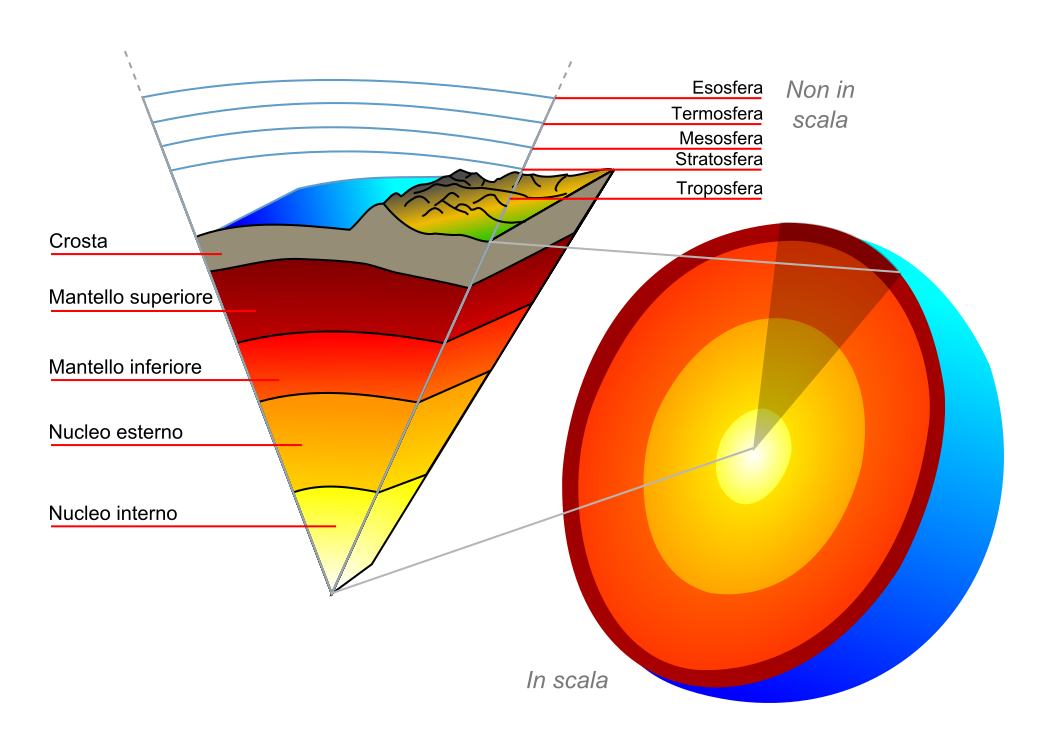
\includegraphics[width=0.50\textwidth]{Chapter-1/crosta-terrestre.png}
\end{wrapfigure}

La terra è composta a strati, o meglio da involucri concentrici (Figura \ref{fig:crostaterrestre}) ed ognuno di essi ha diverse caratteristiche e particolarità.
Al centro della Terra c'è il \textbf{nucleo interno}, ossia un ammasso viscoso composto quasi esclusivamente da ferro avente un raggio di circa 1250 km. Si raggiungono temperature molto elevate, circa 5000-6000$^{\circ}$C.
A seguire abbiamo il \textbf{nucleo esterno}, principalmente composto per il 20\% da ferro e la restante parte nichel, raggiunge circa i 3000$^{\circ}$C. Comprendendo anche il nucleo interno, ha un raggio di circa 3500 km.

Continuando verso l'esterno, troviamo il \textbf{mantello terrestre}, che si divide in superiore ed inferiore.
\\
È composto da diversi metalli ed è difficile stabilire la temperatura dato i moti convettivi del calore, ma si stima intorno ai 500$^{\circ}$C a confine con la crosta terrestre e 3000$^{\circ}$C a confine con il nucleo.
Infine abbiamo la \textbf{crosta terrestre}, che partendo dalla superficie, arriva fino a 70 km di profondità.
Insieme, il \textit{mantello superiore} e la \textit{crosta terrestre} formano la \textbf{litosfera}.
La litosfera è suddivisa in una decina di placche tettoniche principali e altre numerose placche di minori dimensioni (figura 1.2). Queste placche "galleggiano" sullo strato immediatamente sottostante del mantello superiore.\cite{terra}

Esse, data la forte pressione e le alte temperature, subiscono sforzi di enormi dimensioni che formano i \textbf{terremoti}.
I terremoti sono vibrazioni della crosta terrestre, provocate dallo spostamento  di una o più placche nella litosfera.
Le placche si muovono flettendosi lentamente e poi rilasciando (raggiunto il \textit{punto di rottura}) in maniera elastica tutta l'energia accumulata.
Il punto in cui viene generata questa energia è detto \textbf{ipocentro} (2), zona in cui è presente una frattura chiamata \textit{faglia} (3), mentre il punto in superficie posto sulla verticale dell'ipocentro è chiamato \textbf{epicentro} (1).
\begin{figure}[ht]
\label{fig:ipocentro}
\centering
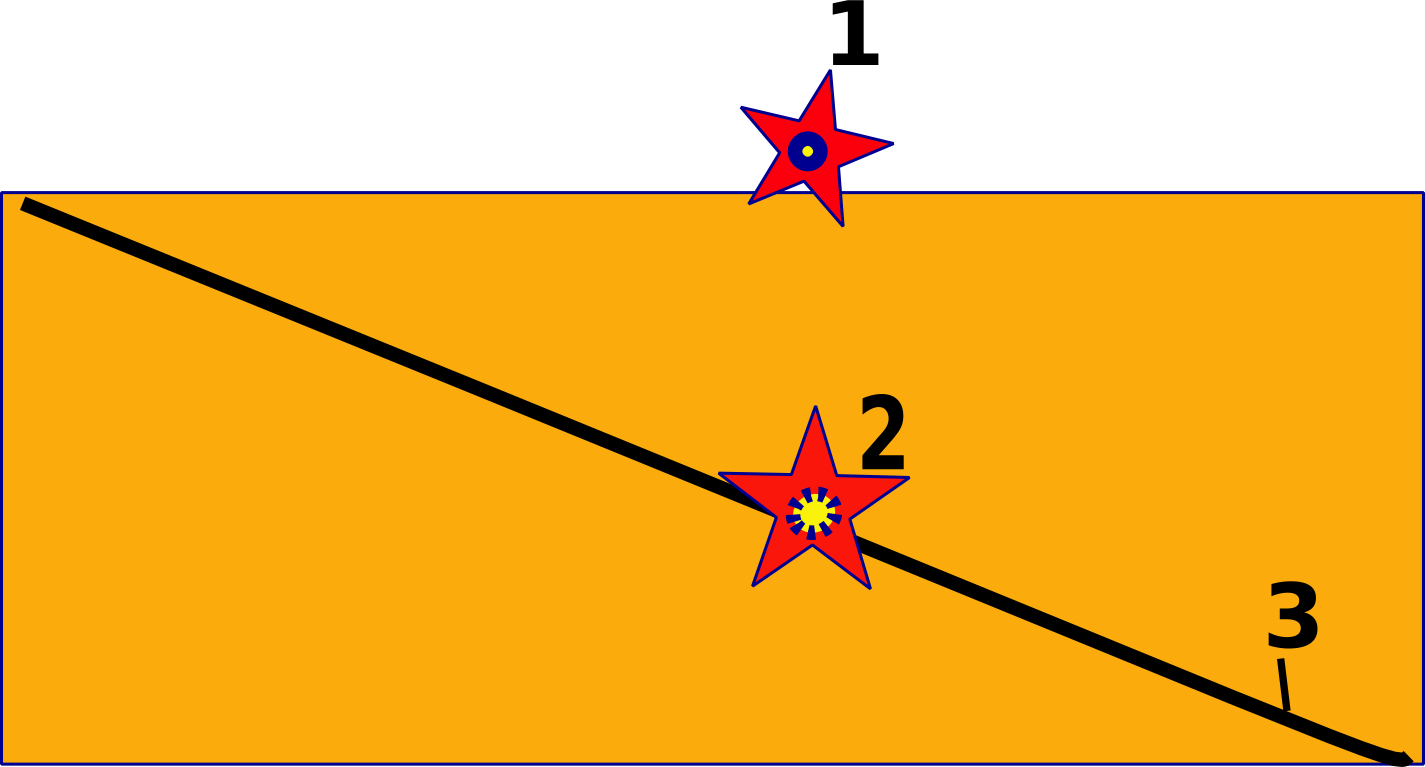
\includegraphics[width=0.55\textwidth]{relazione-tirocinio/Chapter-1/ipo-epi-centro.png}
\end{figure}

\clearpage

\begin{figure}
\caption{Placche tettoniche}
\label{fig:placchetettoniche}
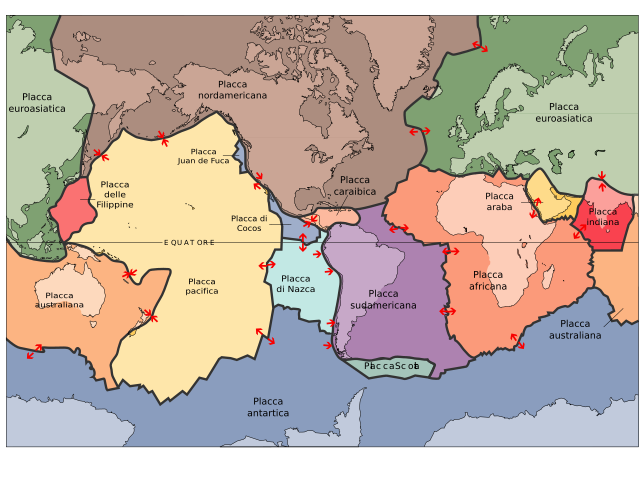
\includegraphics[width=1\textwidth]{Chapter-1/placche-tettoniche.png}
\end{figure}
Esistono tre tipi di faglie: faglie \textit{trascorrenti}, faglie \textit{dirette} e \textit{inverse}.
Esistono in egual numero differenti tipi di onde sismiche.
\\
Le \textbf{onde di compressione o longitudinali} fanno comprimere e dilatare la materia nella stessa direzione con cui si propaga l'onda.
Sono anche dette \textit{primarie}, perché sono le onde che viaggiano a velocità più elevate.
\\
Le \textbf{onde di taglio o trasversali} fanno compiere alla materia oscillazioni in modo perpendicolare alla loro direzione di propagazione. Hanno effetto solo nei solidi, non possono propagarsi attraverso corpi liquidi o gassosi.
Vengono chiamate anche \textit{onde secondarie}, essendo meno veloci delle precedenti.
\\
Le \textbf{onde superficiali}, anche se il nome può essere mal interpretato, non si manifestano in superficie. Questo tipo di onde sono la combinazione delle due precedenti, perciò sono molto complesse e sono le più pericolose. 

\clearpage

\section{Misurazione dei terremoti}

\subsection{Tipologie di terremoti}
Esistono 4 differenti tipologie di terremoti: \textit{tettonici}, \textit{vulcanici}, \textit{da crollo} e \textit{artificiali}.
\\
I terremoti \textbf{tettonici}, come dice il nome, sono provocati dal movimento delle placche tettoniche e hanno origine lungo le faglie.
Sono i più pericolosi ed i più frequenti.
\\
I terremoti \textbf{vulcanici} sono originati dall'attività vulcanica nel sottosuolo. Sono meno pericolosi dei precedenti data la minor energia rilasciata e l'estensione limitata.
\\
I terremoti \textbf{da crollo} si originano durante il crollo di montagne, grotte o frane. Hanno una bassa pericolosità e frequenza.
\\
Infine, i terremoti \textbf{artificiali} vengono originati da attività umane. Ad esempio, una grande esplosione. In generale, hanno una potenza molto limitata.

\subsection{Metodologie di misurazione}
Esistono due tipologie principali di misurazione di un terremoto: la scala \textbf{Mercalli} e la scala \textbf{Richter}.
La scala Mercalli misura l'\textit{intensità} di un terremoto osservando i danni causati da esso. Per questo, dato che tiene in conto solo degli effetti che la scossa produce, può essere applicata anche ai terremoti avvenuti nel passato.
Assegna dei numeri crescenti per intensità, si va dall'uno (impercettebile) sino a dodici (apocalittica).
La scala (o meglio \textit{indice}) Richter misura invece l'energia sprigionata dalla scossa, ossia la \textit{magnitudo}. Viene chiamata scala, ma è più corretto dire indice dato che non ha un range di valori finito. La magnitudo è descritta da questa formula:
\begin{equation*}
  M_w = {\frac{2}{3}}\log_{10}(M_\mathrm{0}) - 10,7
\end{equation*}
dove $M_0$ è il momento sismico all'ipocentro da esprimere in Newton per metro|N·m.\cite{measure}
Ad oggi il massimo valore magnitudo registrato è 9,5.

\subsection{Strumenti di misurazione}
Sono principalmente due: il \textbf{sismografo} ed il \textbf{sismometro}.
Entrambi misurano accelerazione e velocità dei movimenti del suolo, con la differenza che il sismometro misura solamente, ma non può registrare i dati; il sismografo invece oltre alla misura produce anche un grafico temporale, chiamato appunto \textit{sismogramma}.
Uno strumento non può misurare ampie porzioni di territorio, per questo si creano delle reti che monitorano degli ampi spazi di suolo. In Italia questa rete è la \textbf{Rete Sismica Nazionale}.
Con le tecnologie odierne, si utilizzano sismometri digitali insieme ad altri strumenti. Ad esempio, nella rete italiana, le stazioni sono composte da un sismometro, un accelerometro ed una antenna e ricevitore GPS.
È una rete di stazioni sismiche (circa 300) disposte su tutto il territorio italiano e appena fuori dai confini.
Per la maggioranza sono stazioni dell'INGV (Istituto Nazionale di Geologia e Vulcanologia), ma ne fanno parte anche altre piccole reti.
Questa rete monitora sette giorni su sette, 24 ore su 24 i movimenti del suolo e li registra, inviandoli poi ai centri di elaborazione dati di Roma, Grottaminarda e Catania.
La concentrazione maggiore di terremoti in Italia è nell'appennino e nel sud Italia, per questo la maggior parte delle stazioni è posizionata in questi punti, come si può notare nella Figura \ref{fig:RSN}.

\clearpage

\begin{figure}
\caption{Rete Sismica Nazionale \cite{ingv}}
\label{fig:RSN}
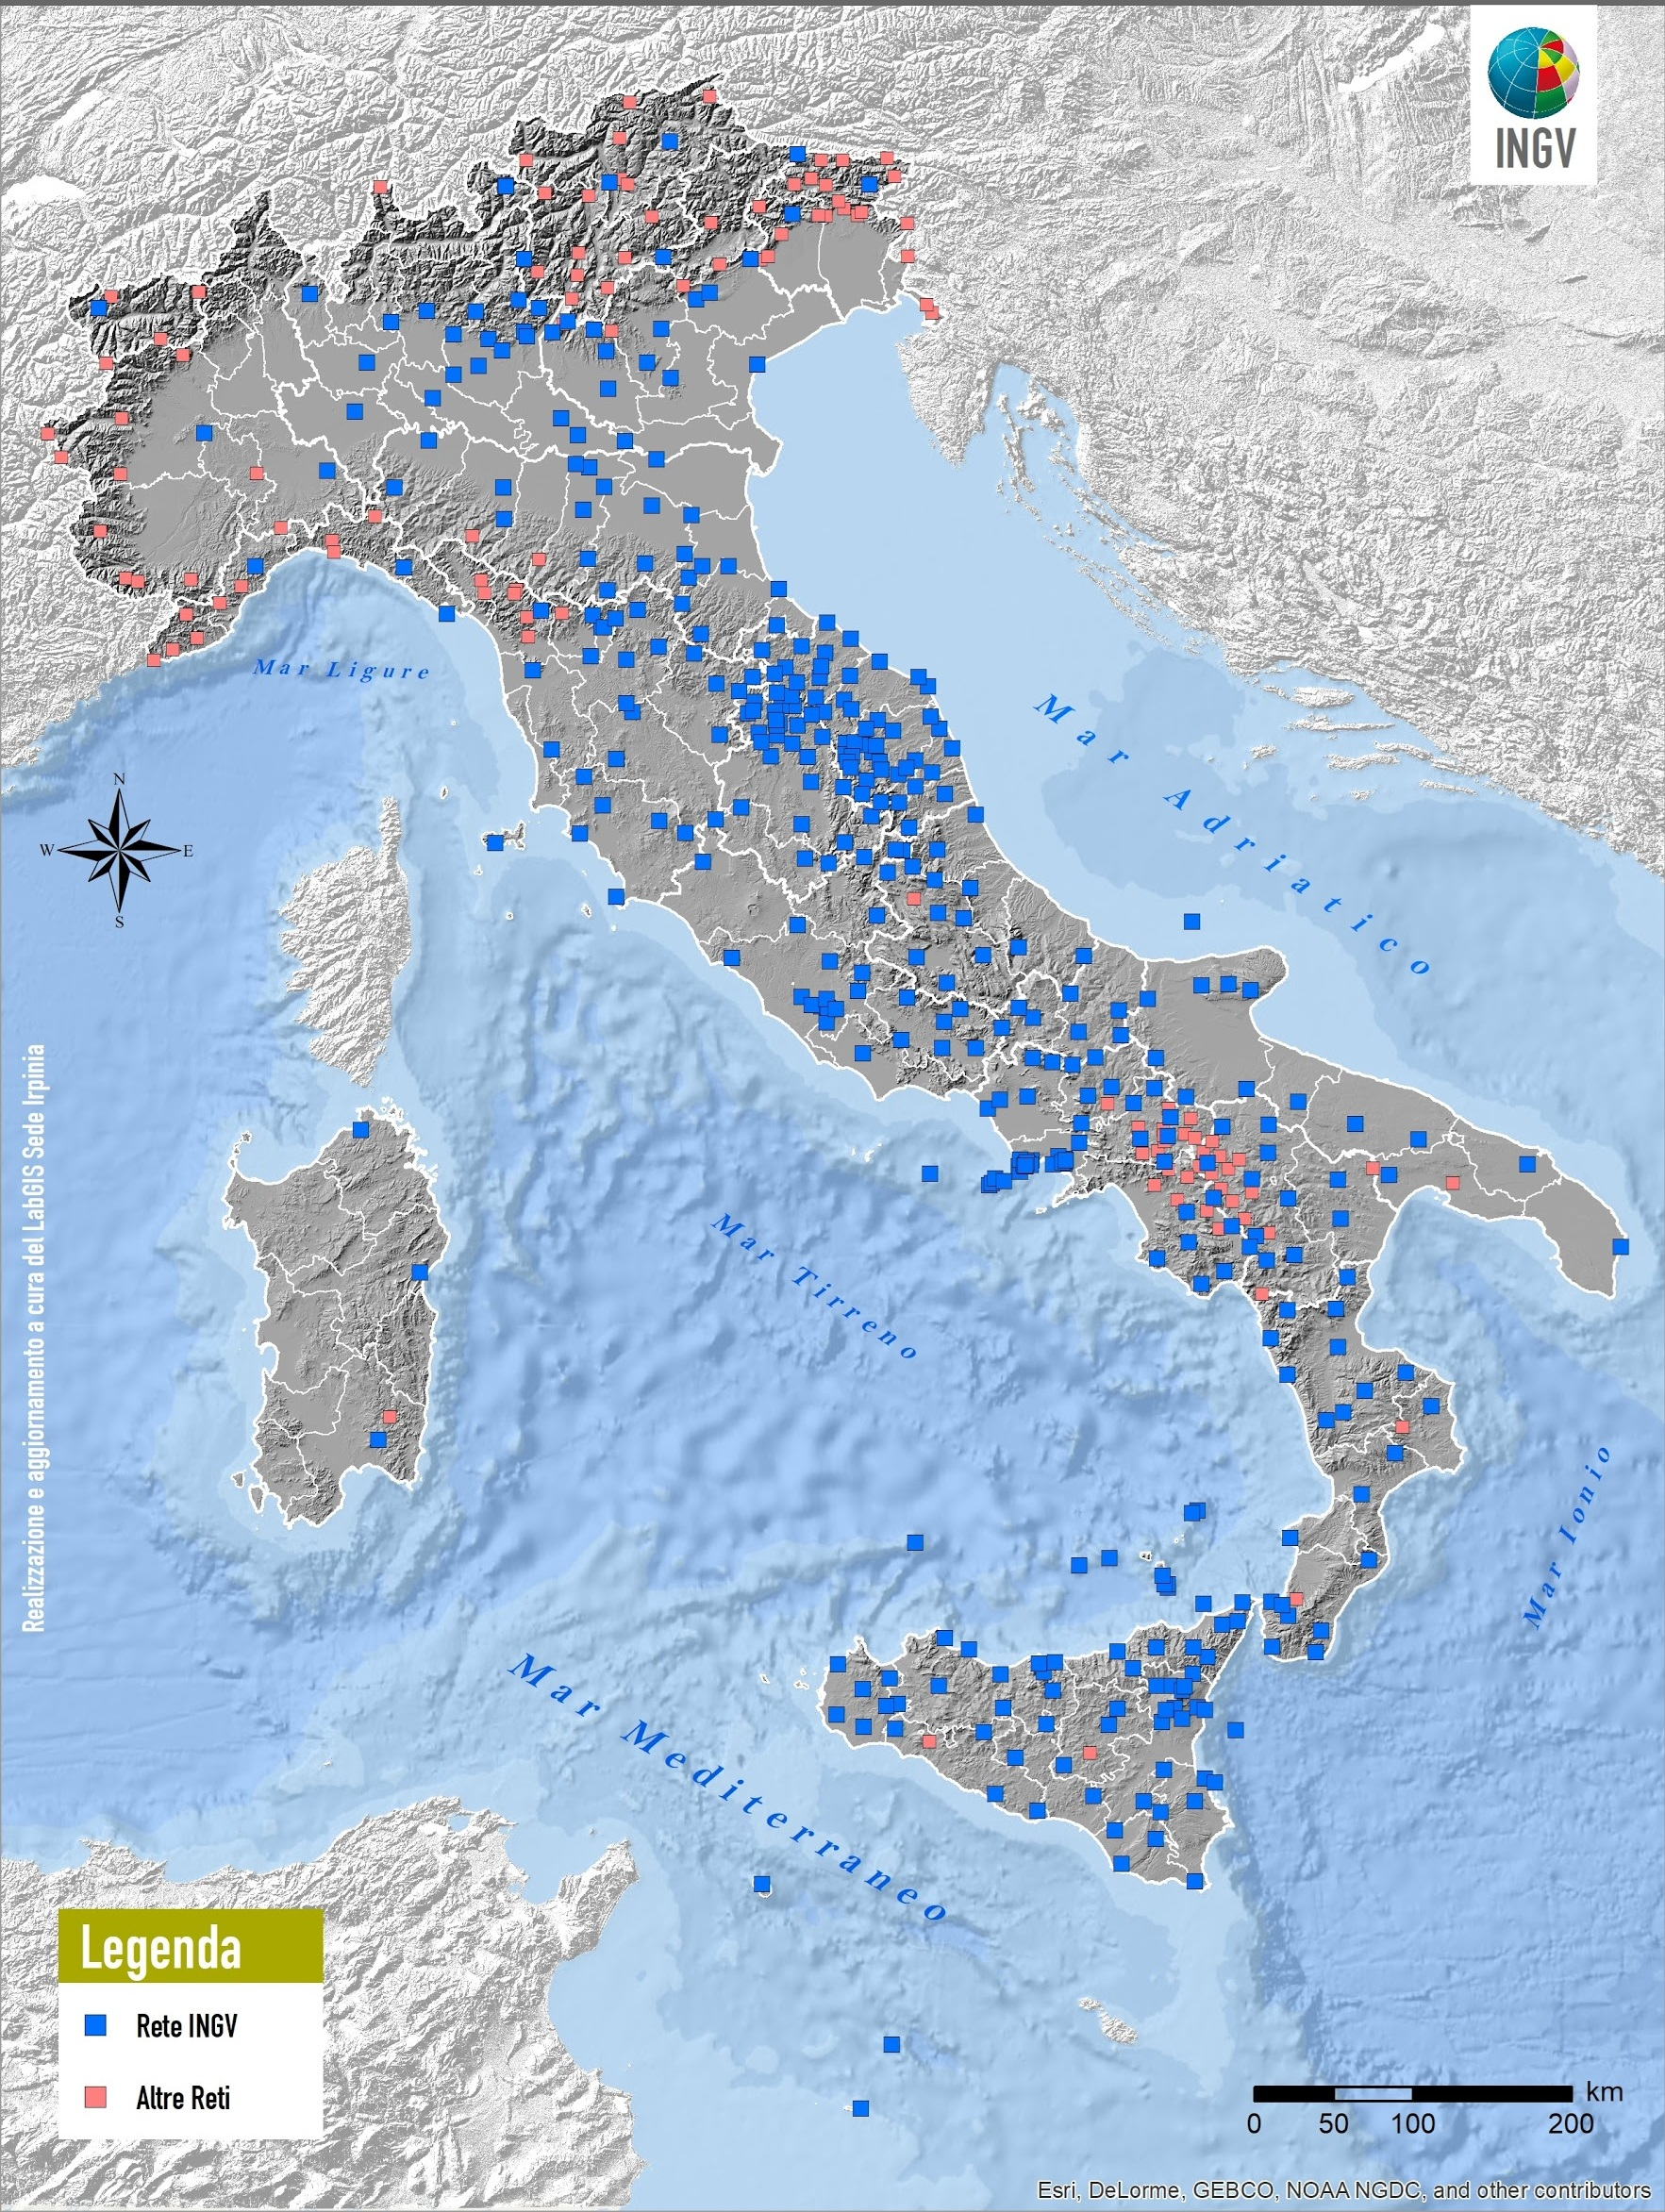
\includegraphics[width=1\textwidth]{Chapter-1/RSN.jpg}
\end{figure}

\clearpage

\section{Piattaforma SeismoCloud}

\subsection{Introduzione al progetto}

\begin{wrapfigure}[14]{r}{0.15\textwidth}

\includegraphics[width=0.15\textwidth]{Chapter-1/seismocloud.png}

\includegraphics[width=0.15\textwidth]{Chapter-1/ingv.jpg}
\end{wrapfigure}

SeismoCloud è una rete di dispositivi IoT (Internet of Things) connessi fra loro a basso costo distribuiti in tutta Italia.
Ha come scopo l'\textit{Earthquake Early Warning}, ossia monitorare l'attività sismica e, nel caso viene rilevato un terremoto, notificare le persone interessate.
L'obiettivo specifico dell'EEW è l'avviso \textbf{in tempo reale} di un possibile sisma.
I sismometri possono essere costruiti personalmente se si ha capacità di elettronica di base, altrimenti viene utilizzato il sensore interno di uno smartphone.
È un progetto nato dall'Università La Sapienza e l'INGV. Viene presentato anche nelle scuole per sensibilizzare gli studenti sul tema terremoti ed
utilizzare questo progetto come
strumento didattico.
Il codice di alcune porzioni di sistema è disponibili su GitHub sotto
l'organizzazione \href{https://github.com/SapienzaApps}{SapienzaApps}.

\subsection{Architettura di sistema}
I sismometri sono di due tipologie: \textit{fissi} e \textit{mobili}.
I \textbf{sismometri fissi} sono dei moduli formati da componenti elettronici a basso costo. Viene usato un chip con un modulo Wi-Fi integrato per la connessione ad Internet, nello specifico il NodeMCU/ESP8266 e un modulo con giroscopio e accelerometro, l'MPU6050.
Sono pensati per essere fissati in modo solidale a muri portanti per una migliore rilevazione.
I \textbf{sismometri mobili} invece utilizzano l'applicazione per smartphone, abilitando l'accelerometro interno del telefono per rilevare vibrazioni.
Devono essere appoggiati su un piano orizzontale, per esempio un tavolo.
Durante la registrazione di un nuovo sismometro fisso, esso viene localizzato per conoscere la sua posizione (fondamentale al rilevamento corretto dei sismi), mentre i sismometri mobili aggiornano di continuano la loro posizione. Nonostante ciò la privacy può essere conservata mostrando il sismometro nella mappa pubblica con una finta posizione casuale nel raggio di 2km.
I sismometri utilizzano il protocollo ISO standard \textbf{MQTT} (Message Queue Telemetry Transport) per inviare e ricevere messaggi di controllo e dati.
\begin{figure}[ht]
\centering
\label{fig:mqtt}
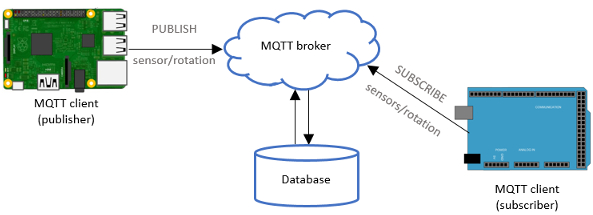
\includegraphics[width=1\textwidth]{Chapter-1/mqtt.jpg}
\end{figure}
Viene utilizzato questo protocollo perché è stato progettato per i dispositivi IoT, dato che questi ultimi hanno, solitamente, una batteria con piccola capienza ed in generale risorse limitate. Rispetto al precedente protocollo HTTP, esso invia messaggi ad alta affidabilità, ha una bassa latenza ed un basso overhead\cite{ottimizzazione}. In MQTT, il \texttt{topic} è una stringa UTF-8 che un broker utilizza per filtrare i messaggi. 
Si può considerare come una etichetta che viene affissa a dei valori che si riferiscono tutti alla stessa cosa. Un broker è il responsabile della comunicazione tra i vari client connessi. I topic hanno una gerarchia basata a livelli. Ogni livello è separato da uno slash. 
Ad esempio il topic che si riferisce alla temperatura del sismometro con identificativo $34$ potrebbe essere \texttt{sensor/34/temperature}.
Dato che MQTT è un protocollo di tipo \textit{publish/subscribe}, i client possono pubblicare dati sun un topic, i quali verranno ricevuti dai client che sono iscritti a quel determinato topic.
I client possono solamente iscriversi ad alcuni topic, oppure solamente pubblicare dati su topic senza iscriversi, oppure possono eseguire entrambe le operazioni.
I dati inviati vengono elaborati in un server centrale che li gestisce, compie dei calcoli su di essi (allo scopo di identificare una possibile scossa di terremoto e lanciare un Earthquake Early Warning) e li archivia.
Come già detto, i dati che i sismometri rilevano vengono salvati in un database. Quando gli utenti richiedono questi dati non viene utilizzato il protocollo MQTT, ma il protocollo HTTP.
Per i messaggi inviati tramite HTTP viene utilizzato lo stile architetturale \textbf{REST} (REpresentational State Transfer).
Questo schema è definito da dei principi \cite{rest}:
\begin{itemize}
  \item Tutto è considerato una risorsa
  \item Ogni risorsa è identificabile da un URI (Uniform Resource Identifier)
  \item Usa metodi HTTP standard (GET, POST, PUT, DELETE)
  \item Possibili rappresentazioni multiple per la stessa risorsa
  \item La comunicazione deve essere sempre senza stato
\end{itemize}
Un esempio di risorsa REST è: \texttt{example.domain/sensor/sensor-id/quake}, dove \texttt{sensor-id} è l'identificatore unico per un sensore.
Tramite l'app mobile (disponibile per Android e iOS) si registrano i nuovi sismometri (sia fissi che mobili). Il sismometro interno viene registrato automaticamente quando viene scaricata l'applicazione per la prima volta. Con i sismometri fissi, quest'ultimo crea una connessione Wi-Fi chiamata \textit{SeismoCloud}. L'utente ci si collega ed inserisce i dati per connettersi alla rete Wi-Fi locale. Successivamente in automatico il dispositivo fisso si collega alla rete Wi-Fi e l'app cerca di trovare nella rete un sismometro.
In entrambi i casi viene richiesto di consentire all'acquisizione della posizione GPS e un nome per il nuovo sismometro.
Attivando un sismometro viene prodotta una mole consistente di dati.
Con una cadenza periodica (qualche minuto, dipende dal carico del sistema) vengono pubblicati: indirizzo IP locale e pubblico, indirizzo MAC e qualità del segnale della rete Wi-Fi, localizzazione e temperatura del sismometro, soglia attuale (valore utile alla rilevazione di una vibrazione).
Quando il sismometro rileva una vibrazione viene inviata l'intensità della vibrazione.
Un topic MQTT è dedicato al comando \textit{reboot}, ossia la possibilità di riavviare il sismometro pubblicando un messaggio.\\
Inoltre è possibile visualizzare la lista dei propri sismometri, una mappa aggiornata in tempo reale con i sismometri attivi e i terremoti recenti, una lista di terremoti con relativa magnitudo, posizione e profondità dell'ipocentro (ordinati cronologicamente) e infine alcuni informazioni utili.
È disponibile anche una interfaccia web è possibile visualizzare tutte le informazioni prima citate ed in più una dashboard personalizzata.
Nella dashboard personale è possibile visualizzare due grafici che mostrano il tempo di utilizzo assoluto e settimanale di ogni sismometro attivo.
Dopo l'effettiva autenticazione (tramite password o QRCode) si entra nella parte privata, ossia relativa ad un determinato \textit{gruppo} (insiemi di sismometri raggruppati per locazione).
Qui, oltre alle funzionalità citate, è presente un sistema di \textbf{EUD} (End User Development).
Dalla pagina Wikipedia \cite{wikieud}:
\begin{quoting}[font=itshape, begintext={``}, endtext={``}]
Lo sviluppo per l'utente finale (EUD) o la programmazione per l'utente finale (EUP) si riferisce ad attività e strumenti che consentono agli utenti finali, persone che non sono sviluppatori di software professionisti, di programmare i computer. Le persone che non sono sviluppatori professionisti possono utilizzare gli strumenti EUD per creare o modificare artefatti software (descrizioni di comportamenti automatizzati) e oggetti di dati complessi senza una conoscenza significativa di un linguaggio di programmazione.
\end{quoting}
Ad esempio, si può ricevere un messaggio automatico tramite Telegram ogni volta che il mio sismometro vibra.

\begin{figure}
\caption{Achitettura di SeismoCloud}
\label{fig:ArchitetturaSeismoCloud}
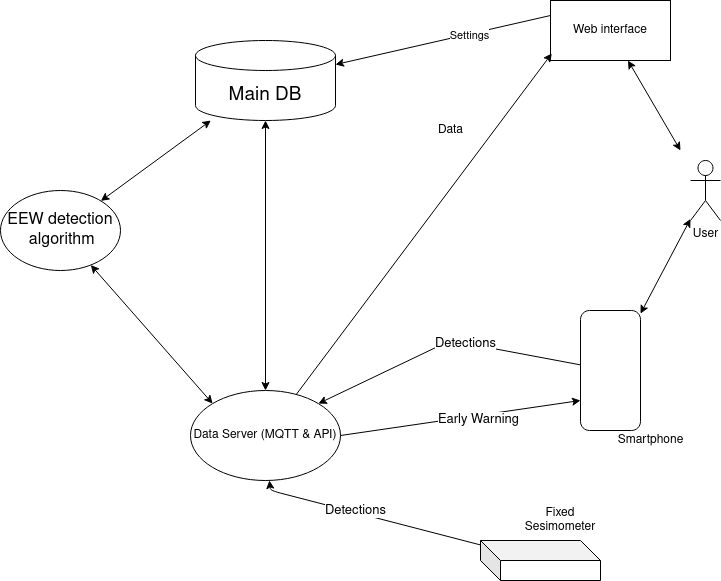
\includegraphics[width=1\textwidth]{Chapter-1/architettura-seismocloud.png}
\end{figure}

\clearpage

\subsection{Un lavoro di gruppo}

\begin{wrapfigure}[14]{r}{0.55\textwidth}
\caption{Rete Sismica SeismoCloud}
\label{fig:RSS}
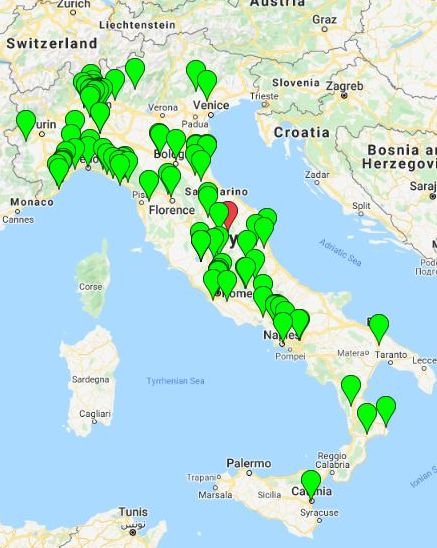
\includegraphics[width=0.55\textwidth]{Chapter-1/seismoitalia.jpg}
\end{wrapfigure}
Come si può notare dalla Figura \ref{fig:RSS} la \textbf{Rete Sismica SeismoCloud} si estende su tutto il territorio nazionale. Si contano circa 100 sismometri attivi.\\
Ad oggi il sistema EEW non è attivo perché i sismometri presenti non bastano a compiere delle rilevazioni sufficienti.

I nodi della rete sono ben distribuiti nel centro Italia, poco nel Sud. Questo è un problema perché l'attività sismica principale in Italia si sviluppa lungo la catena appenninica fino in Sicilia. \\
Grande menzione meritano anche i \\vulcani attivi (Etna, Stromboli, Vesuvio, \\Vulcano).\\

\subsection{Bisogni della community}

\clearpage

% ======================================= CHAPTER 2 ================================================
\chapter{Architettura del sistema}

\section{Sistema Legacy}

Come è stato accennato nella descrizione dell'architettura del sistema (Cap 1.3), è possibile programmare della azioni quando si verificano determinate condizioni.\\
Sostanzialmente le condizioni sono due: quando n sismometri vibrano/sono accesi, oppure la notifica di un Earthquake Early Warning.
Le possibilità per il metodo di notifica sono quattro: un messaggio tramite Telegram, una notifica push ai membri del gruppo, un widget e la pubblicazione di una API.\\

\begin{figure}[H]
\caption{Vecchio sistema EUD}
\label{VecchioEUD}
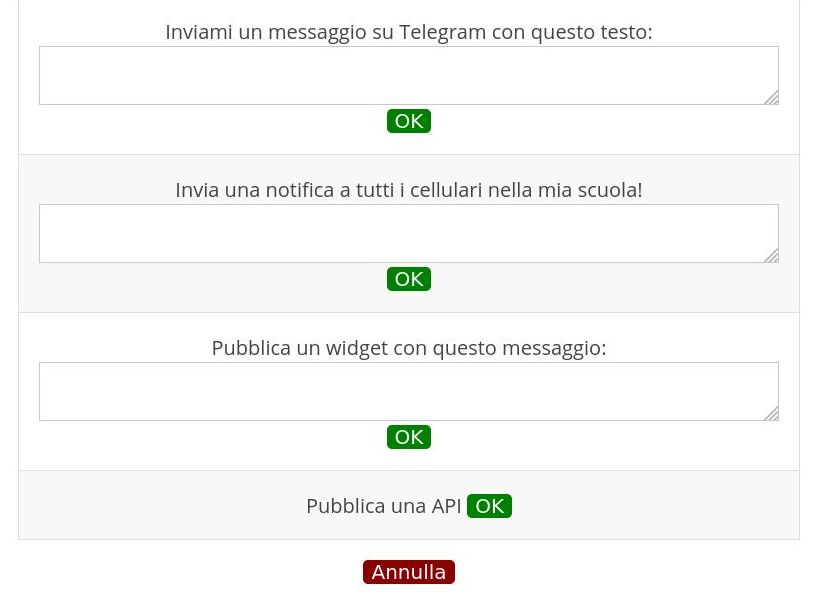
\includegraphics[width=1\textwidth]{Chapter-1/eud-vecchio.jpg}
\end{figure}

Visto che i dati prodotti sono tanti, sarebbe molto utile ampliare il range di condizioni ad un più vasto campo, tenendo in conto anche di tutti i dati che non vengono considerati in questo sistema.

Sarebbe molto più utile lasciare completa \textbf{libertà all'utente} (sotto alcune restrizioni di sicurezza) integrando il sismometro con l'ambiente locale. 

Potrei quindi decidere di riavviare il mio sismometro ogni volta che la temperatura supera i 50$^{\circ}$C. Oppure mandare una mail, pubblicare un tweet e scaricare un file quando vengono rilevate tre vibrazioni nello stesso minuto.

Il tutto non deve risultare complesso, deve essere possibile l'utilizzo per utenti non esperti in informatica o elettronica, ma allo stesso tempo i più competenti devono poter sfruttare le loro abilità.

La soluzione a questo bisogno dovrebbe essere: \textit{facilmente utilizzabile, sicura, affidabile e performante}.

Ad esempio una casa smart con dispositivi IoT o altre tipologie di interazione.

\section{La soluzione proposta: Node-RED}

\subsection{Candidati iniziali}

Piuttosto che progettare e costruire uno strumento di End User Development da zero, si è cercato uno scheletro già pronto e maturo. La ricerca è stata piuttosto semplice, un po' meno la valutazione dei possibili candidati.

Il primo candidato è \textbf{IFTTT} (\href{https://iftt.com}{https://ifttt.com}). È lo strumento più famoso, utilizzato da molte persone, con più di 5 milioni di download su Play Store. Il vantaggio di questa scelta è sicuramente la grande maturità della piattaforma. Gli svantaggi sono la difficoltà nell'integrare i nostri dispositivi con questo sistema, ma soprattutto la somiglianza con il sistema EUD da rimpiazzare, troppo semplice e con condizioni e azioni predefinite.

Una seconda scelta è \textbf{draw.io} (\href{https://app.diagrams.net/}{https://draw.io}). Strumento completamente differente al precedente, è un creatore di diagrammi di flusso. Questo è un tipo di programmazione di azioni che lascia molta libertà all'utente, rimanendo semplice ma efficace. 
\begin{figure}[H]
\caption{Esempio di flusso esportato da draw.io}
\label{fig:drawio}
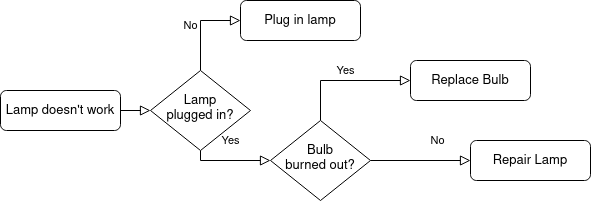
\includegraphics[width=1\textwidth]{relazione-tirocinio/Chapter-2/drawio.png}
\end{figure}
Il codice sorgente di draw.io è disponibile su GitHub. È  ben documentato, quindi questo aiuta l'integrazione con SeismoCloud. Purtroppo si tratta di uno strumento front-end, quindi manca tutta la logica back-end; i dati inseriti dall'utente vengono esportati in file di tipo xml che devono poi essere tradotti in azioni registrate dal sistema. 


\subsection{La piattaforma Node-RED}
Lo strumento che risolve i problemi precedentemente elencati è \textbf{Node-RED} (\href{https://nodered.org}{https://nodered.org}).
Come draw.io è un creatore di diagrammi di flusso ed è anche open-source con repository su GitHub sotto l'organizzazione \href{https://github.com/node-red}{node-red}. È un servizio orientato all'\textit{Internet of Things}, non è uno standard ufficiale, ma è molto utilizzato nel campo.
Qui, a differenza del precedente, esiste uno scheletro back-end, dato che è costruito utilizzando \href{https://nodejs.org}{NodeJS}. Vedremo più avanti in dettaglio come è stato progettato.

La community, oltre ad essere pronta a risolvere dubbi sul forum ufficiale (\href{https://discourse.nodered.org}{discourse.nodered.org}), contribuisce attivamente al progetto implementando delle funzionalità che sono messe a disposizione di tutti tramite il famoso package manager NPM.

Nel nome il 'node' è dato sia dal runtime NodeJS, sia dal nome che hanno gli elementi utilizzati per creare i flussi, chiamati appunto \textit{nodi}.
\begin{figure}[H]
\caption{Esempio flusso di nodi in Node-RED}
\label{fig:node-red-flows-example1}
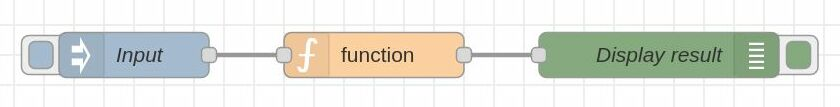
\includegraphics[width=1\textwidth]{relazione-tirocinio/Chapter-2/node-red-flows-1.jpg}
\end{figure}
Come si nota in figura \ref{fig:node-red-flows-example1}, i nodi sono dei rettangoli che hanno funzioni particolari:
\begin{itemize}
    \item \textbf{Nodi input}: Questi nodi emettono valori e non prendono nulla in ingresso, quindi sono utilizzati per produrre dati o iniziare dei flussi. Possono avere da 1 a n valori in uscita.
    \item \textbf{Nodi intermedi}: Sono nodi che hanno sia input che output. Sono utilizzati per applicare delle funzioni ai dati in ingresso, oppure il dato in ingresso viene solamente utilizzato per far iniziare una procedura intermedia. Prendono in input un solo valore e possono avere da $1$ a $n$ valori in uscita.
    \item \textbf{Nodi output}: Sono gli opposti dei nodi input. Non hanno valori in uscita ma solo in ingresso. Sono utilizzati per terminare un flusso, solitamente sono quindi le azioni da effettuare nel caso in cui si verificano le condizioni stabilite. Possono avere un solo valore in ingresso.
\end{itemize}
\begin{figure}[H]
\caption{Esecuzione del comando shutdown}
\label{fig:node-red-flows-example2}
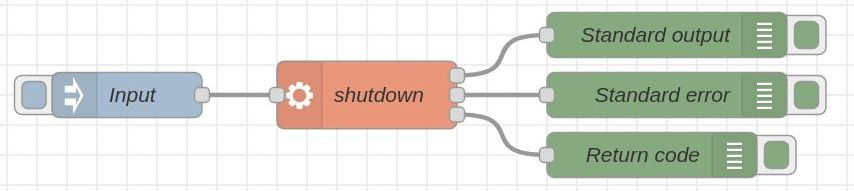
\includegraphics[width=1\textwidth]{relazione-tirocinio/Chapter-2/node-red-flows-2.jpg}
\end{figure}
Nella figura \ref{fig:node-red-flows-example2} abbiamo un altro esempio. Qui quando viene cliccato il pulsante a sinistra del nodo \textit{input}, il nodo invia in uscita un valore (in questo caso qualsiasi, ad esempio 3 o la stringa 'input') che fa eseguire il secondo nodo (di tipo \textit{intermedio}). Il nodo \textit{shutdown} esegue il comando `shutdown` e stampa nella console di debug lo stdout, stderr ed il return code.

Data la facilità d'uso, il grande supporto (repository con 10+K star su GitHub, community molto attiva e forum ufficiale), la maturità del progetto (versione 0.2 nel 2013, ad oggi (2020) 1.1.3), la facile estendibilità ed integrazione con dispositivi IoT (come appunto i nostri sismometri), decisamente Node-RED è lo strumento più adatto per risolvere i bisogni della community SeismoCloud.

\clearpage

\section{Implementazione di Node-RED per SeismoCloud}

\subsection{Come funziona Node-RED}
Può essere utilizzato in vari modi, ad esempio: su un computer in locale, tramite Docker, su un dispositivo Raspberry, oppure su alcuni sistemi Cloud (IBM Cloud, Amazon Web Services, Microsoft Azure).

L'interazione con l'utente avviene tramite un browser web. 

Un \textbf{nodo} è il blocco costruttivo di base di un flusso. Le funzionalità dei nodi sono scatenate da eventi esterni (richieste HTTP o altro protocollo oppure un timer) o da input ricevuti da altri nodi. Processano il messaggio ricevuto oppure ne creano uno nuovo e possono inviare messaggi ai nodi successivi nel flusso. 

Un \textbf{nodo di configurazione} è un tipo speciale di nodo che setta delle configurazioni utili agli altri nodi, ma non fa parte di nessun flusso. Ad esempio, i nodi \textit{MQTT-in} e \textit{MQTT-out} utilizzano il nodo di configurazione \textit{MQTT-broker} che rappresenta una connessione condivisa con un broker MQTT.

Un \textbf{flusso} è rappresentato da un tab o foglio di lavoro ed è il metodo principale per organizzare il lavoro. Informalmente un flusso rappresenta un insieme di nodi connessi fra loro.

Un \textbf{sottoflusso} è una collezione di nodi che vengono collassati graficamente in un unico nodo. Possono essere utilizzati per ridurre la complessità grafica del flusso, oppure per riutilizzare un gruppo di nodi più volte in un flusso.
\begin{figure}[H]
\caption{Esempio di sottoflusso}
\label{fig:sottoflusso}
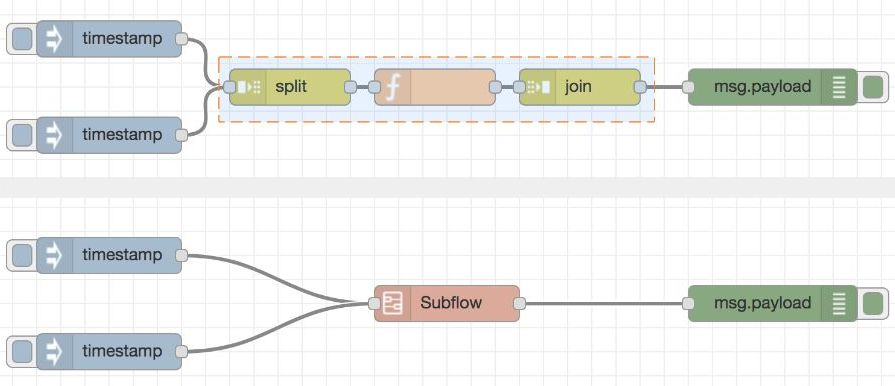
\includegraphics[width=1\textwidth]{relazione-tirocinio/Chapter-2/node-red-flows-4.jpg}
\end{figure}
Il \textbf{contesto} è il modo principale di condividere informazioni tra i nodi senza essere connessi fra loro. Ne esistono di tre tipi:
\begin{itemize}
    \item Node: Visibile solamente dal nodo che setta il valore
    \item Flow: Visibile a tutti i nodi che appartengono allo stesso flusso (o tab)
    \item Global: Visibile a tutti i nodi
\end{itemize}
Un \textbf{messaggio} è un oggetto JSON che viene passato attraverso i nodi. Di default si chiama \textit{msg} ed ha due campi: \textit{payload} e \textit{id}. 

La \textbf{palette} è posizionata sulla sinistra dell'interfaccia e lista tutti i nodi presenti nel sistema. Dei nodi extra possono essere aggiunti direttamente dall'editor.

Il \textbf{workspace} è lo spazio principale, dove tutti i nodi vengono posizionati in modo da creare degli automatismi.

La \textbf{sidebar} è uno spazio posizionato a destra del workspace in cui ci sono degli strumenti utili, ad esempio la console di debug, l'interfaccia della configurazione dei nodi e la finestra descrittiva per ogni nodo.


È molto orientato al riuso ed alla portabilità, infatti tutti i nodi o collezioni di nodi sono moduli Javascript che possono essere caricati e utilizzati poi da altri tramite NPM.

Inoltre, ogni flusso viene poi tradotto in codice JSON per poter essere esportato ed importato in altri ambienti.

Viene fornita anche una 'vetrina' (\href{https://flows.nodered.org}{flows.nodered.org}) dove possono essere esplorati nodi e flussi creati e pubblicati per la community.

Esempio di un semplice flusso Node-RED:
\begin{figure}[H]
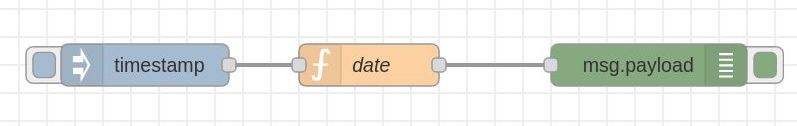
\includegraphics[width=1\textwidth]{relazione-tirocinio/Chapter-2/node-red-flows-3.jpg}
\end{figure}
Il nodo \textit{date} non è altro che un nodo function che restituisce la data:
\begin{lstlisting}[language=JavaScript]
// Create a Date object from the payload
var date = new Date(msg.payload);
// Change the payload to be a formatted Date string
msg.payload = date.toString();
// Return the message so it can be sent on
return msg;
\end{lstlisting}
Viene tradotto in JSON:
\begin{lstlisting}[language=JavaScript]
[
    {
        "id":"58ffae9d.a7005",
        "type":"debug",
        "name":"",
        "active":true,
        "complete":false,
        "x":640,"y":200,
        "wires":[]
    },
    {
        "id":"17626462.e89d9c",
        "type":"inject",
        "name":"timestamp",
        "topic":"",
        "payload":"",
        "repeat":"",
        "once":false,
        "x":240,
        "y":200,
        "wires":[["2921667d.d6de9a"]]
    },
    {
        "id":"2921667d.d6de9a",
        "type":"function",
        "name":"date",
        "func":"// Create a Date object from the payload\nvar date = new Date(msg.payload);\n// Change the payload to be a formatted Date string\nmsg.payload = date.toString();\n// Return the message so it can be sent on\nreturn msg;",
        "outputs":1,
        "x":440,
        "y":200,
        "wires":[["58ffae9d.a7005"]]
    }
]
\end{lstlisting}
Dato che Node-RED ha tutti i dati in-memory, per salvare i flussi creati utilizza (di default) un file chiamato \textit{flows.json}. Questo rende molto facile condividere i progetti.

\subsection{Progettazione ************MODIFICARE**********}
Il vecchio sistema di EUD rende possibile, come già introdotto, la programmazione di azioni condivisa con il proprio gruppo di appartenenza.

Questa impostazione viene ripresa nel nuovo sistema, quindi ogni membro di un gruppo deve poter accedere alla propria \textit{istanza di gruppo di Node-RED} per programmare le azioni desiderate con tutti e soli i dati dei sismometri appartenenti al gruppo.

La ragione principale di questa scelta è che in questo modo si hanno molti più dati disponibili. Infatti, in media ogni gruppo ha una decina di sismometri attivi.

\clearpage

\subsection{Vantaggi nell'utilizzo di Docker}

Lo strumento che più soddisfa i requisiti imposti è \textbf{Docker}.
È uno dei sistemi più noti per il deployment di applicazioni software, incapsula i programmi all'interno di contenitori astraendo dal sistema operativo sottostante.
Utilizza i \textit{container}, cioè un insieme di più processi isolati dal resto del sistema.
I container sono utili perché sono altamente portabili in tutti gli ambienti e restano integri dallo sviluppo ai test.

Viene costruita un'immagine, ossia un file chiamato Dockerfile, che definisce tutte le dipendenze ed i file necessari per creare un container.
Una immagine Docker consiste in livelli read-only i quali rappresentano istruzioni Docker. Una istruzione aggiunge qualcosa al livello precedente.


Esempio di Dockerfile:
\begin{lstlisting}[language=Javascript]
FROM ubuntu:18.04
COPY . /app
RUN make /app
CMD python /app/app.py
\end{lstlisting}

Ogni istruzione crea un livello:

\begin{itemize}
    \item FROM crea un livello dall'immagine Docker di ubuntu versione 18.04
    \item COPY aggiunge i file dalla cartella corrente del Docker client
    \item RUN costruisce l'applicazione con make
    \item CMD specifica quale comando eseguire nel container
\end{itemize}
Quando viene eseguita un'immagine e generato un container, si aggiunge un ulteriore livello sopra ai precedenti.

Tutte le modifiche poi fatte al container in esecuzione sono eseguite su questo nuovo livello.

Viene fornita l'immagine di base ufficiale di Node-RED scaricabile dalla repository di DockerHub (\href{https://hub.docker.com/r/nodered/node-red/}{https://hub.docker.com/r/nodered/node-red/}).

\begin{lstlisting}[language=docker]
# from nodered/node-red:1.0.6-12
FROM nodered/node-red@sha256:82f367ab41d19e3ebd5e9b1cc62e4f615d4b4be4fa8bc83f1bf5441ba8c0d32a

# Qui vengono settate tutte le variabili d'ambiente
ENV VAR="hello-world"

# Vengono creati i volumi per la persistenza dei dati
VOLUME /volume

# Tutte le cartelle vengono copiate nell'immagine
COPY data data

RUN chown -R node-red data
USER node-red

RUN npm install #Tutti i nodi custom necessari

CMD ["npm", "start"]
\end{lstlisting}
\clearpage

La persistenza dei dati viene garantita dal volume (nell'esempio chiamato appunto volume). 

È una parte del file-system che viene riservata per salvare i dati prodotti dal container in esecuzione.

Questo garantisce che se il container va in uno stato di errore o la macchina dove viene deployato il container si spegne, i dati vengono comunque salvati in un disco fisso.


Differisce dalla \textbf{virtualizzazione} in:

\begin{itemize}
    \item Deployment semplificato: permette di impacchettare l'applicativo in un singolo elemento distribuibile
    \item Ampia portabilità: i container possono essere creati, distrutti e replicati in qualsiasi ambiente in modo semplice e veloce
    \item Prestazioni: Sono più leggeri e veloci delle macchine virtuali perché non hanno una emulazione del sistema operativo virtuale
\end{itemize}

\begin{figure}[H]
\caption{Container vs Virtualizzazione}
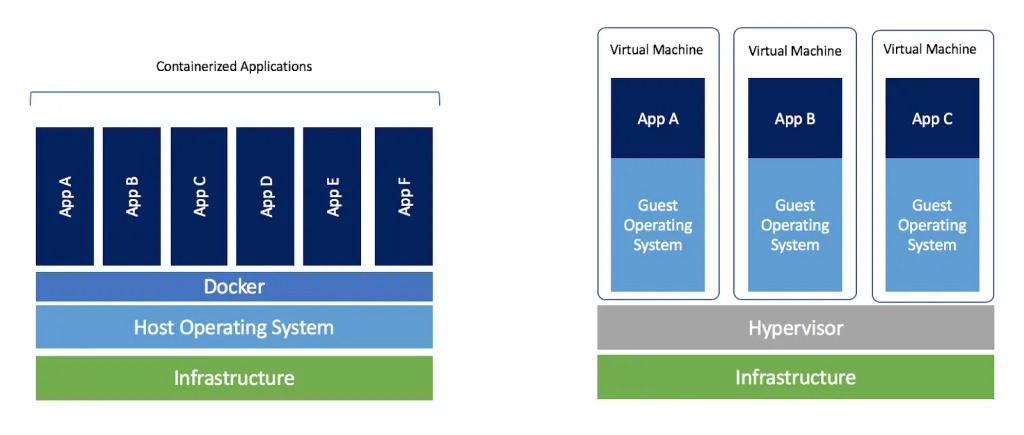
\includegraphics[width=1\textwidth]{relazione-tirocinio/Chapter-2/vm-c.jpg}
\end{figure}
Questa divisione netta fra i container si presta molto al nostro caso. Ogni container avrà in esecuzione una instanza di node-red configurata con i dati di un determinato gruppo.

Dato che ogni container è isolato, non ci sono problemi di dati condivisi fra i vari gruppi.


Come si può notare dai grafici nelle prossime pagine, nello studio "Performance Evaluation of Docker Container and Virtual Machine" (di Amit M. Potdara, Narayan D. G., Shivaraj Kengond e Mohammed Moin Mulla), ci sono molti vantaggi prestazionali nell'utilizzare i container Docker invece di macchine virtuali.

Come viene scritto sul paper, \begin{quoting}[font=itshape, begintext={``}, endtext={``}]
Le prestazioni computazionali possono essere misurate dal numero di operazioni che il sistema performa in un dato tempo (eventi/sec) o dal tempo di completamento di un certo compito. I risultati maggiormente dipendono dal numero di core della CPU virtuale che è allocata nel server. La comparazione nei test delle prestazioni della CPU è stato fatta utilizzando gli strumenti sysbench, Phoronix e Apache benchmark.
\end{quoting}

\begin{figure}
    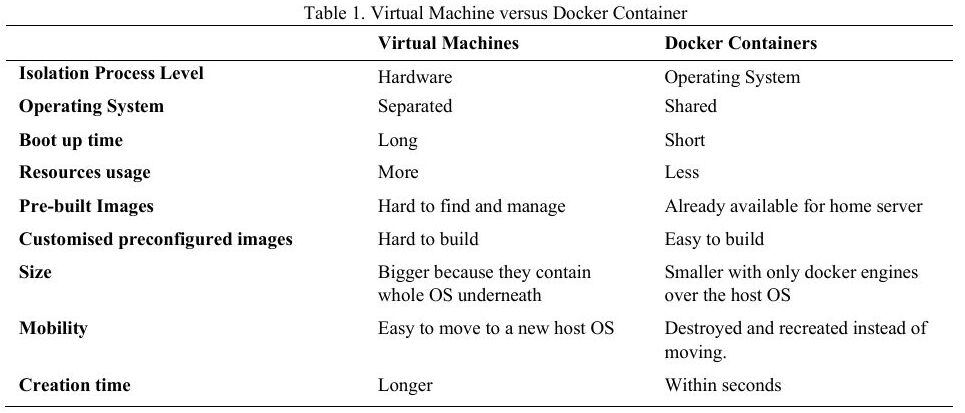
\includegraphics[width=1\textwidth]{relazione-tirocinio/Chapter-2/docker-vm-1.jpg}
    \label{fig:docker-vm-1}
\end{figure}
Sono state comparate le prestazioni della CPU, come già anticipato sopra, con Sysbench. È stato utilizzato il metodo \textbf{Massimo numero primo}.

Viene dato un tempo massimo, in questo caso 60 secondi e deve essere dato in risultato il numero primo massimo minore di 50000 con 4 thread operativi.

Per il test di compressione dati è stato utilizzato 7-Zip con un file di 10GB.

le prestazioni della memoria RAM (utilizzando RAM speed/SMP) e un caso particolare. Come caso particolare è stato utilizzato Eigth Queen, una simulazione di un problema del gioco degli scacchi. 
\begin{figure}
\begin{tabular}{cc}
  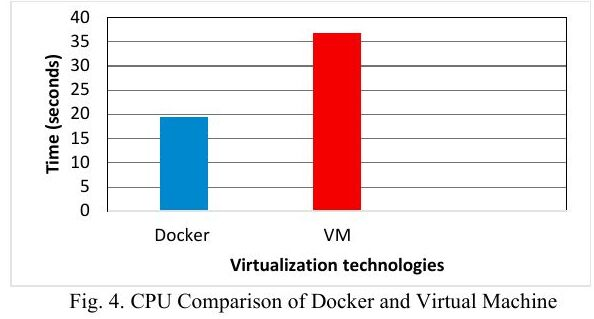
\includegraphics[width=0.5\textwidth]{relazione-tirocinio/Chapter-2/docker-vm-2.jpg} &   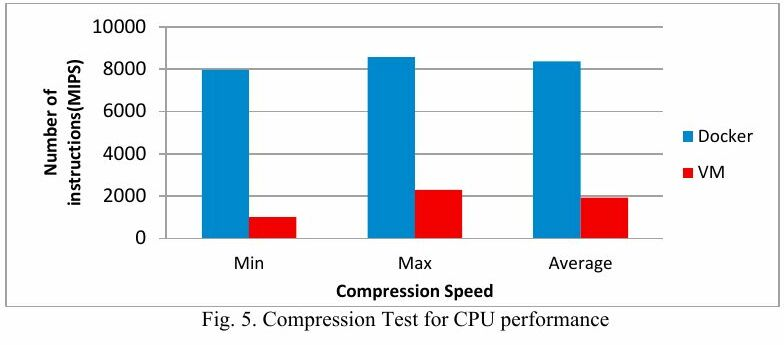
\includegraphics[width=0.5\textwidth]{relazione-tirocinio/Chapter-2/docker-vm-3.jpg} \\
 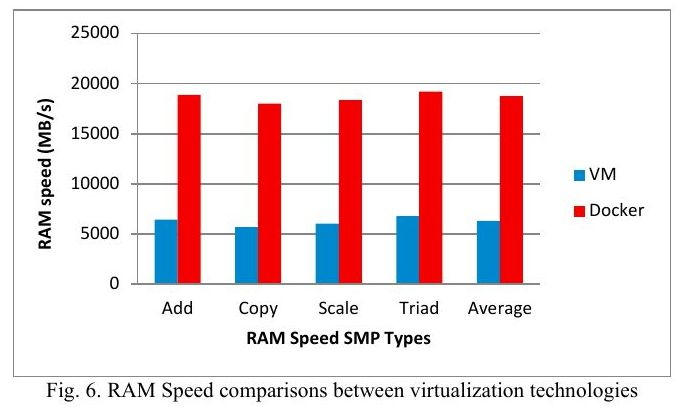
\includegraphics[width=0.5\textwidth]{relazione-tirocinio/Chapter-2/docker-vm-4.jpg} &   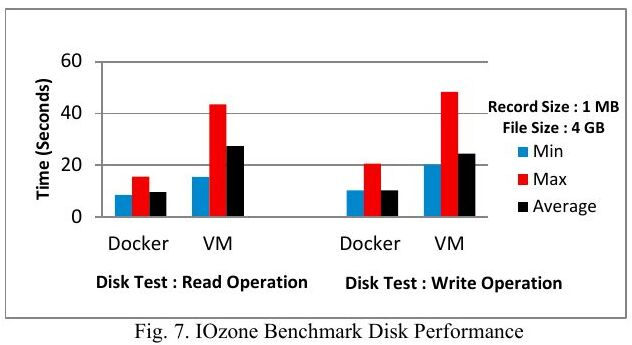
\includegraphics[width=0.5\textwidth]{relazione-tirocinio/Chapter-2/docker-vm-5.jpg} \\
\end{tabular}
\end{figure}

\clearpage


\subsection{Schema finale architettura}
\begin{figure}[H]
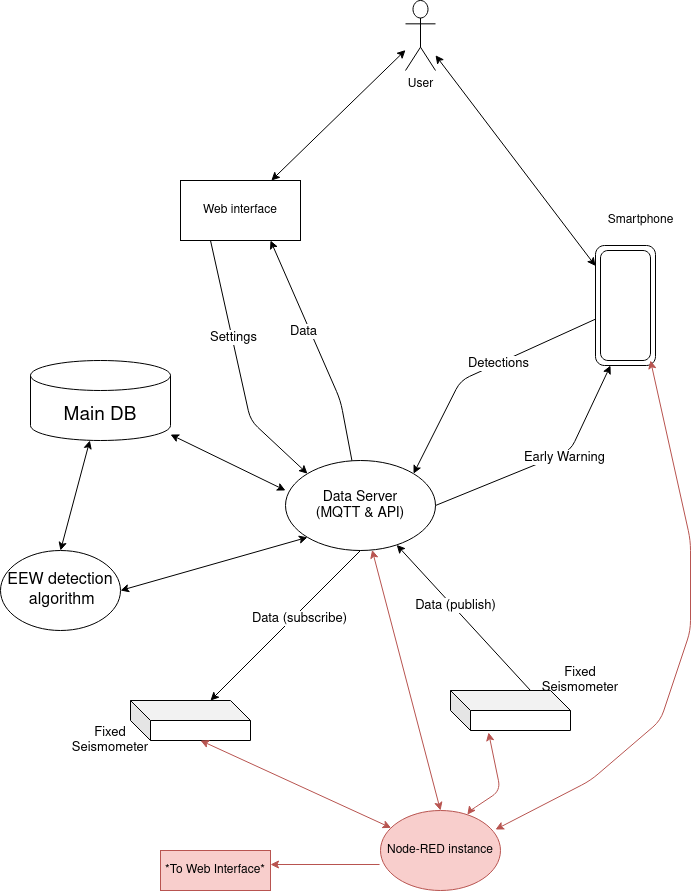
\includegraphics[width=1\textwidth]{relazione-tirocinio/Chapter-2/architettura-seismocloud2.png}
\end{figure}

\clearpage

Qui con \textbf{node-RED instance} si intende un container per un gruppo specifico.

Il container interagisce con l'interfaccia web riguardo tutta l'interazione con l'utente.

Interagisce con i sismometri attraverso i vari protocolli per lo scambio di dati (HyperText Transfer Protocol, Message Queue Telemetry Transport ...)

Interagisce con gli smartphone nel caso in cui gli utenti decidono di ricevere notifiche o altri tipi di alert su telefoni cellulari (tipo messaggi telegram).

Con il data server scambia informazioni con il broker mqtt e riceve informazioni sul gruppo (statistiche e dati dei sismometri) attraverso le API.


Il deploy di tanti servizi può essere semplificato utilizzando \textbf{docker-compose}.

\begin{lstlisting}[language=docker-compose-2]
version: '3'
services:

  seismocloud-nodered-1:
    restart: always
    image: seismocloud-nodered:latest
    environment:
      - NUM_GROUP = 2222345435
    ports:
      - 1880:1880
    volumes:
      - ./volume:/volume
      
  seismocloud-nodered-2:
    restart: always
    image: seismocloud-nodered:latest
    environment:
      - NUM_GROUP = 2222345436
    ports:
      - 1880:1880
    volumes:
      - ./volume:/volume
\end{lstlisting}
Compose è uno strumento per definire ed eseguire applicazioni Docker multi-container.

In questo caso appunto, vengono eseguiti due servizi node-red con immagine customizzata (seismocloud-nodered) per due differenti gruppi.

Con un singolo comando si possono eseguire tutti i servizi configurati in precedenza (\textit{docker-compose up}), oppure stopparli (\textit{docker-compose stop}) e con un altro farli ripartire (\textit{docker-compose restart}).

Se, mentre tutti i servizi sono in esecuzione, si vuole modificare lo stato di uno solo è possibile farlo con i comandi di Docker.
\clearpage

% ======================================= CHAPTER 3 ================================================
\chapter{Implementazione delle funzionalità}

\section{Difficoltà e limiti nell'uso di Node-RED}

placeholder

\clearpage

\section{Implementazione delle funzionalità tramite nodi}

placeholder

\clearpage

\section{Ottimizzazione delle prestazioni}

placeholder

\clearpage

% ======================================= CHAPTER 4 ================================================
\chapter{Sicurezza e protezione dei dati}

\section{Sicurezza nella piattaforma Node-RED}

placeholder

\clearpage

\section{Ricerca ed analisi di vulnerabilità}

placeholder

\clearpage

\section{Risoluzione dei problemi}

placeholder

\clearpage


% ======================================= CHAPTER 5 ================================================
\chapter{Test, conclusioni e sviluppi futuri}

\section{Iterazioni dei Test}

placeholder

\clearpage

\section{Conclusioni}

placeholder

\clearpage

\section{Sviluppi futuri}

placeholder

\clearpage

\refstepcounter{chapter}

\chapter*{Ringraziamenti}

\cleardoublepage

\refstepcounter{chapter}

% ======================================= BIBLIOGRAPHY ================================================
\begin{thebibliography}{9}

\bibitem{terra}
  \textbf{Stuttura interna della terra}.\\
  \href{https://it.wikipedia.org/wiki/Struttura_interna_della_Terra}{https://it.wikipedia.org/wiki/Struttura\_interna\_della\_Terra}

\bibitem{measure}
  \textbf{Earthquake Magnitude, Energy Release, and Shaking Intensity}.\\
  \href{https://www.usgs.gov/natural-hazards/earthquake-hazards/science/earthquake-magnitude-energy-release-and-shaking-intensity}{https://www.usgs.gov/natural-hazards/earthquake-hazards/science/earthquake-magnitude-energy-release-and-shaking-intensity}

\bibitem{ingv}
  \textbf{Istituto Nazionale di Geologia e Vulcanologia}.
  \href{http://ingv.it}{http://ingv.it}

\bibitem{ottimizzazione}
  \textbf{Ottimizzazione delle risorse nell’uso di servizi in background in SeismoCloud per Android}.
  \href{https://github.com/Enrico204/bachelor-degree-thesis}{https://github.com/Enrico204/bachelor-degree-thesis}

\bibitem{berkeleyfaq}
  \textbf{Seismo Berkeley Lab FAQ}.
  \href{http://seismo.berkeley.edu/outreach/faq.html}{http://seismo.berkeley.edu/outreach/faq.html}

\bibitem{rest}
  \textbf{REST API documentation}.
  \href{https://restfulapi.net/}{https://restfulapi.net/}

\bibitem{wikieud}
  \textbf{Wikipedia - End User Development}.
  \href{https://en.wikipedia.org/wiki/End-user_development}{https://en.wikipedia.org/wiki/End-user_development}

\bibitem{MathWorks}
  \textbf{Publish MQTT messages and subscribe to message topics}.\\
  \href{https://www.mathworks.com/help/supportpkg/raspberrypi/ref/publish-and-subscribe-to-mqtt-messages.html}{https://www.mathworks.com/help/supportpkg/raspberrypi/ref/publish-and-subscribe-to-mqtt-messages.html}

\bibitem{noderedwiki}
  \textbf{Node-RED Wiki}.
  \href{https://github.com/node-red/node-red/wiki}{https://github.com/node-red/node-red/wiki}

\bibitem{nodereddoc}
  \textbf{Node-RED Documentation}.
  \href{https://nodered.org/docs}{https://nodered.org/docs}

\bibitem{dockerdoc}
  \textbf{Docker Documentation}.
  \href{https://docs.docker.com/}{https://docs.docker.com/}

\bibitem{dockervsvm}
    \textbf{Performance Evaluation of Docker Container and Virtual Machine}
    \\
    \href{https://www.sciencedirect.com/science/article/pii/S1877050920311315}{https://www.sciencedirect.com/science/article/pii/S1877050920311315}

\bibitem{dockerfilesbestpractices}
    \textbf{Best practices for writing Dockerfiles}
    \\
    \href{https://docs.docker.com/develop/develop-images/dockerfile_best-practices/}{https://docs.docker.com/develop/develop-images/dockerfile\_best-practices/}

\end{thebibliography}

\end{document}